\section{Background}
\label{sec:compiler:background}

In this section, we briefly review \cc{}'s memory model and memory relations (\Cref{sec:compiler:background:compcert}) and interaction semantics of \ccc{} (\Cref{sec:compiler:background:isem}).

\subsection{CompCert's Memory Model and Memory Relations}
\label{sec:compiler:background:compcert}

\myparagraph{Undefined Behavior}
UBs can be understood as erroneous (forbidden) operations, so that compilers are licensed to translate them into arbitrary behaviors.
A typical example of such erroneous operation is buffer overrun, which may spoil the stack frame, and thus invalidate basic assumptions compiler has made.
Note that compilers are not required to detect those UB -- it is impossible to detect it statically, and doing so dynamically will give too much overhead.
Instead, programmers are obligated to avoid UB, and compilers can optimize assuming the source program is free of UB.

To capture those intuitions, UB is formally defined as a set of all possible behaviors.
Recall that the semantics preservation (\Cref{sec:rusc:background}) property states that behaviors of the source program includes that of the target.
By defining UB this way, compilers are indeed licensed to translate UB into arbitrary behaviors.
Also, programmers are indeed obligated to avoid UB, because if UB is executed then anything can happen (\eg{}leaking private data).

%% As mentioned in \Cref{sec:overview:compiler}, UBs can be understood as forbidden behaviors, so that compilers are licensed to translate them into any behaviors.

\myparagraph{\cc{} Memory Model}
{\it Memory model} determines, for each memory operations, how the memory is changed and what are the return values.

The simplest way to define a memory model is to represent memory as a single large map, just as in hardware.
This model is often called {\it flat} (or {\it concrete}) memory model.
Formally, the model is defined as follows.
\[
\begin{array}{r@{~~}c@{~~}l}
\textrm{Mem} & \defeq & \texttt{uint32} \rightarrow \option{\textrm{Val}} \\ %\mathbb{N}
\textrm{Val} & \defeq & \texttt{uint32}
\end{array}
\]
Note that both pointer and integer values are represented as a 32-bit integer in $\textrm{Val}$.
%% Note that $\textrm{Val}$ is just a 32-bit integer, which means both pointer and integer values are represented as a mere natural number.
$\textrm{Mem}(p) = \some{v}$ means that the location $p$ is allocated and it contains a value $v$. On the other hand, $\textrm{Mem}(p) = \none$ means it is not allocated yet.


However, flat memory model does not properly model buffer overrun as UB, and thus it cannot validate essential compiler translations.
Specifically, see the following example:
\begin{figure}[h]
\begin{minipage}{1.2\linewidth}
\begin{minipage}{0.60\linewidth}
\begin{Verbatim}[frame=single]
int main() {            int main {
  int* x = malloc(4);     int* x = malloc(4);
  x[0] = 0;               x[0] = 42;
  f();               -->  f();
  out(x[0]);              out(42);
}                       }
\end{Verbatim}
\end{minipage}
\hspace*{-2.7mm}
\begin{minipage}{0.3\linewidth}
\begin{Verbatim}[frame=single]
int f() {
  int* y = malloc(4);
  y[1] = 43;
}


\end{Verbatim}
\end{minipage}
\end{minipage}
%% \makebox[\linewidth]{\makebox[1.2\linewidth]{
%% }}
\caption{A counterexample showing the problem with flat memory model}
\label{fig:flat-model}
\end{figure}

%% In this example, if the address of \begin{verbatim}x\end{verbatim} and \begin{verbatim}y+4\end{verbatim} happens to be the same, the translation is invalid because the source prints 43 and while the target prints 42.
%% The root cause of the problem is that there is no way to distinguish the two pointer \begin{verbatim}x\end{verbatim} and \begin{verbatim}y+4\end{verbatim}, where the former should be allowed to access \begin{verbatim}x[0]\end{verbatim} while the latter should not.
\noindent In this example, if the address of x and y+4 happens to be the same, the translation is invalid because the source prints 43 while the target prints 42.
The root cause of the problem is that there is no way to distinguish two pointer x and y+4 where the former should be allowed to access x[0] while the latter should not.


To address this problem, \cc{} uses a different memory model that is also called {\it logical} memory model.
Conceptually, in this model memory consists of a finite set of blocks where each block is an array of finite size.
It is formally defined as follows (simplified for presentation purpose):
\[
\begin{array}{r@{~~}c@{~~}l}
%% \textrm{Mem} & \defeq & \{ (m, nb) \in (Block \rightarrow \mathbb{Z} \rightarrow (\textrm{Perm} \times \textrm{Val})) \times \textrm{Block} \} \\
\textrm{Mem} & \defeq & \{ (m, nb) \in (Block \rightarrow \mathbb{Z} \rightarrow (\textrm{Perm} \times \textrm{Val})) \times \textrm{Block} \; | \; \\
%% & & \;\;\; \forall \; b, o, p, v, m(b, o) = (p, v) \land p \eq \textrm{Invalid} \implies b < nb \} \\
& & \;\;\; \forall \; b, o, v, m(b, o) = (\textrm{Valid}, v) \implies b < nb \} \\
%% \textrm{Mem} & \defeq & \{ (m, nb) \; | \; (m \in Block \rightarrow \mathbb{Z} \rightarrow (\textrm{Perm} \times \textrm{Val})) \land (nb \in \textrm{Block}) \} \\
%% \textrm{Mem} & \defeq & \{ ((m \in Block \rightarrow \mathbb{Z} \rightarrow (\textrm{Perm} \times \textrm{Val})), (nb \in \textrm{Block})) \} \\
\textrm{Block} & \defeq & \texttt{uint32} \\
\textrm{Val} & \defeq & \texttt{uint32} \uplus (\textrm{Block} \times \mathbb{Z}) \uplus \Undef \\
%% \textrm{Perm} & \defeq & \textrm{Valid} \uplus \textrm{Nonempty} \uplus  \textrm{Invalid} \\
\textrm{Perm} & \defeq & \textrm{Valid} \uplus \textrm{Invalid} \\
%% \textrm{Perm} & \defeq & \textrm{Allocated} \uplus  \textrm{Unallocated} \\
\end{array}
\]
If a block's permission (\textrm{Perm}) is \textrm{Valid}, then it is an allocated block and accessible. If it is \textrm{Invalid}, then it is not allocated yet or already freed, thus accessing it is considered UB.
Values are either a 32-bit integer, a pointer composed of a block id and an offset inside it, or an \Undef value which can be understood as an uninitialized value. %% pair $(b,o)$ where $b$ is a block id and $o$ is an offset inside it.
In $\textrm{Mem}$, for a given address $(b,o)$, $m$ returns permission and the value contained in that address.
$nb$ (which is an abbreviation of next block) always points to the smallest fresh block id. Therefore, whenever a memory is allocated, it increments $nb$ by one and returns $(nb, 0)$.

With logical memory model, the above translation is valid.
Note that $x$ and $y$ originates in different allocations, so they have different block id.
Therefore, one cannot access $x$ with $y$ no matter the offset.
Actually, accessing $y[1]$ executes UB because its permission is \textrm{Invalid}, so the semantic preservation holds trivially.


%% where each block corresponds to each allocation of the program.
%% \cc{}'s memory model consists of a finite set of blocks of finite size
%% and a pointer value (or, an address) is a pair $(b,o)$ of a block id $b$ and an offset $o$ inside it.
%% The memory identity imposes that the source and target memories are identical;
%% and the extension that the two memories contain identical block ids and
%% each target block extends the corresponding source block
%% with more space and any values in it at the end.

\myparagraph{Memory Relations of \cc{}}
\label{sec:overview-verification:injection:original}
As previously mentioned, \cc{} uses three memory relations: identity, extension, and injection.
The memory identity imposes that the source and target memories are identical;
and the extension that the two memories contain identical block ids and
each target block extends the corresponding source block
with more space and any values in it at the end.

A memory injection injects a subset of the source blocks into target blocks
without overlap. More precisely, a (selected) whole source block is injected into a single target block
while allowing multiple source blocks to be injected into the same target block without overlap.
This injection map specifies the \emph{public} areas of the source and target memories and the correspondence between them.
In other words, the corresponding addresses by the injection map are treated as \emph{equivalent} (public) pointer values,
%% and therefore
so that at those corresponding addresses,
only equivalent%
\footnote{Technically speaking, \cc{} allow more undefined values in the source
  because it proves refinement rather than equivalence between the source and target programs.}
values (\ie equivalent non-pointer values or corresponding addresses) should be stored .
All the areas that are not on the injection map are considered as \emph{private} areas of the source and target memories.


\hide{
We briefly review those memory relations with focus on injection, the most sophisticated one.

The memory identity imposes that the source and target memories are identical, which is defined as follows.
\[
\begin{array}{l@{~~}c@{~~}l}
m_{src} & = & m_{tgt} \\
nb_{src} & = & nb_{tgt} \\
v_{src} & = & v_{tgt} \\
\end{array}
\]

The memory extension imposes that the two memories contain identical block ids and each target block extends the corresponding source block with more space and any values in it. Formally,\\
%% \forall \; b, o, (m_{src}(b, o), m_{tgt}(b, o)) &\in& \{\; (p_{src}, v_{src}), (p_{tgt}, v_{tgt}) \;|\; \lessdef{p_{src}}{p_{tgt}} \land \lessdef{v_{src}}{v_{tgt}} \;\} \\
\hspace{-6mm}$ \forall \; b, o, (m_{src}(b, o), m_{tgt}(b, o)) \in \{ (p_{src}, v_{src}), (p_{tgt}, v_{tgt}) \,|\, \lessdef{p_{src}}{p_{tgt}} \;\land\; \lessdef{v_{src}}{v_{tgt}} \} $\vspace{-2mm}
\[
\hspace{20mm}\begin{array}{r@{~~}c@{~~}l}
nb_{src} & = & nb_{tgt} \\
v_{src} & \lessdefsymbol & v_{tgt} \\
\textrm{where } \lessdef{p_{src}}{p_{tgt}} & \defeq & p_{src} = \textrm{Invalid} \;\lor\; p_{src} = p_{tgt} \\
\textrm{and } \lessdef{v_{src}}{v_{tgt}} & \defeq & v_{src} = \Undef \;\lor\; v_{src} = v_{tgt}
\end{array}
\]
%% \textrm{     where } $\lessdef{p_{src}}{p_{tgt}} \defeq p_{src} = \textrm{Invalid} \;\lor\; p_{src} = p_{tgt}$,
%% \textrm{     and } $\lessdef{v_{src}}{v_{tgt}} \defeq v_{src} = \Undef \;\lor\; v_{src} = v_{tgt}$.

%% The memory identity imposes that the source and target memories are identical; and the extension that the two memories contain identical block ids and each target block extends the corresponding source block with more space and any values in it at the end.
A memory injection injects a subset of the source blocks into target blocks
without overlap. More precisely, a (selected) whole source block is injected into a single target block
while allowing multiple source blocks to be injected into the same target block without overlap.
This injection map specifies the \emph{public} areas of the source and target memories and the correspondence between them.
In other words, the corresponding addresses by the injection map are treated as \emph{equivalent} (public) pointer values,
%% and therefore
so that at those corresponding addresses,
only equivalent%
\footnote{Technically speaking, \cc{} allow more undefined values in the source
  because it proves refinement rather than equivalence between the source and target programs.}
values (\ie equivalent non-pointer values or corresponding addresses) should be stored.
All the areas that are not on the injection map are considered as \emph{private} areas of the source and target memories.

\cc{} uses a simpler relation whenever possible to simplify the correctness proof.
Specifically, memory identity
}

\myparagraph{Memory Relations of \ccm{}}
\label{sec:overview-verification:injection}

%% Now we 

\ccm{} uses the original memory identity and extension of \cc{}
(\Cref{sec:overview-verification:injection:original}) and mildly
strengthens the original memory injection to reason about dynamically allocated
local memory such as a function's stack frame for \emph{open} modules,
which can be compared to the structured injection of \ccc{}
(\Cref{sec:overview-verification:injection:dynamic}).
Moreover, we generalize it further to reason about statically allocated local memory
such as static variables of C by allowing module-local invariants on those static variables
(\Cref{sec:overview-verification:injection:static}).

%% and mildly generalize the memory injection of \cc{} in two steps: first to reason
%% about dynamic local memory such as a function's stack frame
%% (\Cref{sec:overview-verification:injection:dynamic}) and further to
%% reason about static local memory such as static variables of C
%% (\Cref{sec:overview-verification:injection:static}).
%% Structured injections of \ccc{} can be compared to our first generalization






\subsection{Interaction Semantics}
\label{sec:compiler:background:isem}

We give a brief overview of interaction semantics of \ccc{}, which
interactively executes modules equipped with their own independent
module semantics. Each module semantics $M$ provides
a set of module states (also called \emph{cores}) $\States{M}$ with the following operations:
\begin{itemize}
\item \texttt{init\_core}: given a function $f$ with arguments $\vec{v}$,
  %and a memory $m$,
  gives the initial module state $s \in \States{M}$
  % with updated memory $m'$
  executing the invoked function $f$ with $\vec{v}$.
\item \texttt{at\_external}: given $s \in \States{M}$,
  %and a memory $m$,
  checks if an external function $f$ is called with arguments~$\vec{v}$.
  %% and if so, gives updated memory $m'$ and state $s'$.
\item \texttt{after\_external}: given $s \in \States{M}$
  where an external function is called,
  %a memory $m$
  and a return value $r$,
  gives the module state $s'$
  %and memory $m'$
  after the function call returns $r$.
\item \texttt{halted}: given $s \in \States{M}$, checks if the module execution is halted with a return value~$r$.
\item \texttt{corestep}: given $s \in \States{M}$ and memory $m$, takes a local step producing an event $e$ and the next state~$s'$ with updated memory $m'$.
\end{itemize}

We explain how interaction semantics works using an example in
\Cref{fig:inter-sem}, where the whole machine state consists of a
memory, say $m$, and a stack of module states (called \emph{core stack}), say $[s_2; s_1]$.
Then, interaction semantics checks whether the stack-top module $s_2$
is invoking an external function using \texttt{at\_external}, and if
so, pushes the invoked module's initial state, say $s_3$, obtained by
\texttt{init\_core}. Note here that the same module $M_1$ can have
multiple module states $s_1$ and $s_3$ in the stack.  Then the
new top module $s_3$ takes a local step to $s_3'$ with updated memory
$m'$ according to its \texttt{corestep}, and if $s_3'$ is a halted
state with a return value $r$ (checked with \texttt{halted}), the top
module $s_3'$ is popped and returned to the next module $s_2$, which
is then updated to $s_2'$ given by \texttt{after\_external} with the return
value $r$.

\begin{figure}[t]
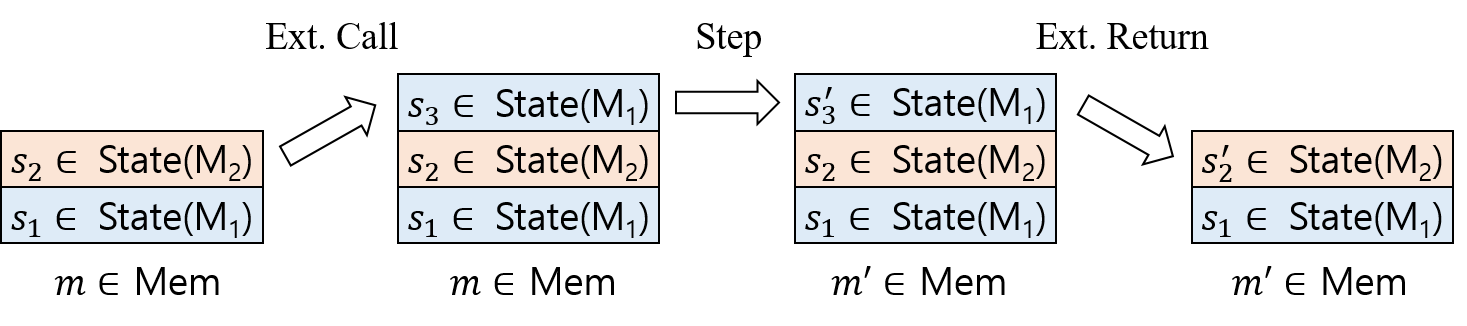
\includegraphics[width=0.9\linewidth]{images/intersem.png}
\caption{An execution of interaction semantics}
\label{fig:inter-sem}
\end{figure}

%% marshalling unmarshalling
%% marshalling the argument values into a list of values
%% setting the initial core states, unmarshalling the list of arguments.
%% at\_external: marshalling the argument values into a list of values
%% after\_external: unmarshalling the return value into
%% halted: marshalling the return value
%% corestep: use the underlying language semantics

Finally, note that the language semantics of C, assembly and
intermediate languages can be lifted to give a module semantics by
defining \texttt{corestep} to be the same as the execution step of the
language's semantics, and the other module operations to reflect the
calling conventions. Note also that all language-specific resources
(\ie other than the memory)
such as the register-file of assembly 
reside inside the module state, and thus are
duplicated at each invocation of a module.

%% One can lift a \cc{} language semantics into a core semantics by providing the interfaces:
%% Note that it is possible to define a core semantics using a mathematical specification.
